\documentclass[sigconf,nonacm]{acmart}

\usepackage{booktabs}
\usepackage{graphicx}

\setcopyright{none}
\copyrightyear{2026}
\acmYear{2026}
\acmDOI{}
\acmConference[CS410 Tech Review]{Technical Review Project}{May 05, 2026}{Urbana, IL}
\acmISBN{}

\begin{document}

\title{Technical Review of ColBERTv2 Retrieval with RAGatouille on SciFact}

\author{Kaiyu Liu}
\email{kaiyul3@illinois.edu}
\affiliation{%
  \institution{University of Illinois Urbana-Champaign}
  \city{Urbana}
  \state{Illinois}
  \country{USA}
}

\author{Yuyang Zeng}
\email{yuyang16@illinois.edu}
\affiliation{%
  \institution{University of Illinois Urbana-Champaign}
  \city{Urbana}
  \state{Illinois}
  \country{USA}
}

\renewcommand{\shortauthors}{Liu and Zeng}

\begin{abstract}
This technical review evaluates ColBERTv2, a late-interaction neural retrieval
model, through the RAGatouille Python library. We compare ColBERTv2 against an
Okapi BM25 baseline on the BEIR SciFact benchmark and study the effect of
ColBERT residual-compression bit width on retrieval quality, index size, build
time, and query latency. The review focuses on both retrieval effectiveness and
the practical engineering work needed to reproduce ColBERT-style retrieval in a
small scientific claim-search setting.
\end{abstract}

\keywords{Information Retrieval, ColBERT, RAGatouille, BM25, SciFact, Late Interaction}

\maketitle

\section{Introduction}

Retrieval-augmented systems depend on a retriever that can find relevant
evidence even when a query and a document do not share exact words. BM25 remains
a strong sparse baseline because it is simple, fast, and interpretable, but it
cannot directly model semantic matches. ColBERTv2 addresses this gap with
contextual token embeddings and a late-interaction scoring function that keeps
many of BERT's semantic benefits while avoiding a full cross-encoder pass over
every query-document pair.

This review studies whether RAGatouille makes ColBERTv2 practical for a course
scale reproduction study. Our experiment uses SciFact, where claims must retrieve
scientific abstracts that support or refute them.

\section{Background}

\subsection{BM25}

BM25 ranks documents using lexical term matching with document-length
normalization. It is a useful first-stage baseline because it requires no
training data and can index small corpora quickly.

\subsection{ColBERTv2 and Late Interaction}

ColBERT encodes each query and document independently into token-level vectors.
At search time, each query token finds its maximum-similarity document token,
and those maximum scores are summed. This MaxSim operation allows fine-grained
semantic matching while keeping document representations indexable.

\subsection{RAGatouille}

RAGatouille wraps ColBERT indexing, search, and reranking behind a smaller
Python API. In this project, it is used to build PLAID indexes for SciFact and
to expose ColBERT as a retriever that can be evaluated like a standard TREC run.

\section{Methods}

\subsection{Dataset}

We use BEIR SciFact. The test split contains 300 queries and a 5,183-document
corpus of scientific abstracts. Queries are scientific claims; qrels map each
claim to relevant abstracts.

\subsection{Systems}

The BM25 baseline uses \texttt{rank\_bm25} with lowercasing, stopword removal,
and default Okapi parameters \texttt{k1=1.5} and \texttt{b=0.75}.

The ColBERT system uses the \texttt{colbert-ir/colbertv2.0} checkpoint through
RAGatouille. We build separate indexes for \texttt{nbits} values 1, 2, and 4 to
measure the residual-compression trade-off. The implementation records both the
requested \texttt{nbits} and the effective \texttt{nbits} observed in the
underlying ColBERT configuration.

\subsection{Metrics}

We report NDCG@10, MRR@10, MAP, and Recall@100 using \texttt{ranx}. We also
record index size, index build time, total search time, and p50/p95 query
latency. Statistical comparisons use paired Student's t-tests over per-query
metric vectors with Holm-Bonferroni correction.

\section{Results}

Table~\ref{tab:retrieval} shows that ColBERTv2 improves over BM25 on all four
retrieval metrics. The largest absolute gain is on Recall@100, where ColBERTv2
retrieves relevant abstracts for more claims in the top-100 candidates. The
NDCG@10 gain is smaller but directionally consistent with the expected benefit
of semantic late interaction.

\begin{table}[h]
  \centering
  \caption{Retrieval effectiveness on BEIR SciFact test.}
  \label{tab:retrieval}
  \begin{tabular}{lrrrr}
    \toprule
    System & NDCG@10 & MRR@10 & MAP & Recall@100 \\
    \midrule
    BM25 & 0.6641 & 0.6317 & 0.6251 & 0.8759 \\
    ColBERTv2, nbits=1 & 0.6924 & 0.6693 & 0.6623 & 0.9120 \\
    ColBERTv2, nbits=2 & 0.6924 & 0.6693 & 0.6623 & 0.9120 \\
    ColBERTv2, nbits=4 & 0.6924 & 0.6693 & 0.6623 & 0.9120 \\
    \bottomrule
  \end{tabular}
\end{table}

The paired tests show that the BM25-to-ColBERT deltas are positive but not
statistically significant after Holm-Bonferroni correction. For the default
\texttt{nbits=2} comparison, the NDCG@10 delta is +0.0283
($p=0.1148$), and the MRR@10 delta is +0.0376 ($p=0.0540$). The MRR confidence
interval is barely positive, but it does not survive the multiple-comparison
correction used in this review.

\subsection{Residual-Compression Ablation}

Table~\ref{tab:latency} reports the index and latency measurements for
\texttt{nbits} values 1, 2, and 4. The requested and effective bit widths
matched for all runs, so the ablation is exercising the intended ColBERT
configuration. However, all three settings produced identical ranking metrics
and identical measured index sizes in this small SciFact setup.

\begin{table}[h]
  \centering
  \caption{Index footprint and latency for ColBERTv2 variants.}
  \label{tab:latency}
  \begin{tabular}{rrrrr}
    \toprule
    nbits & Index MiB & Build s & p50 ms & p95 ms \\
    \midrule
    1 & 84.95 & 1092.6 & 63.1 & 188.0 \\
    2 & 84.95 & 1284.5 & 69.2 & 76.5 \\
    4 & 84.95 & 1261.4 & 66.4 & 77.8 \\
    \bottomrule
  \end{tabular}
\end{table}

\begin{figure}[h]
  \centering
  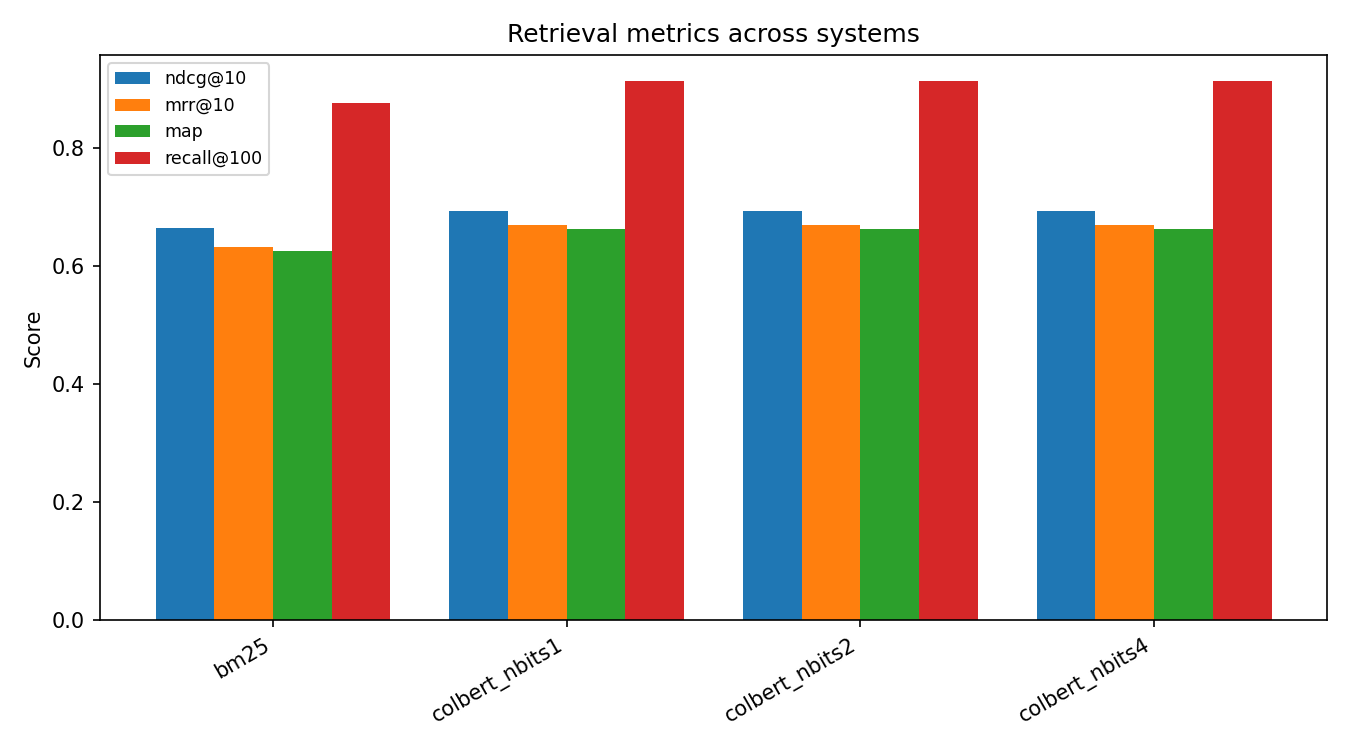
\includegraphics[width=\linewidth]{../results/figures/metrics_bar.png}
  \caption{Retrieval metrics across BM25 and ColBERTv2 variants.}
  \label{fig:metrics}
\end{figure}

\begin{figure}[h]
  \centering
  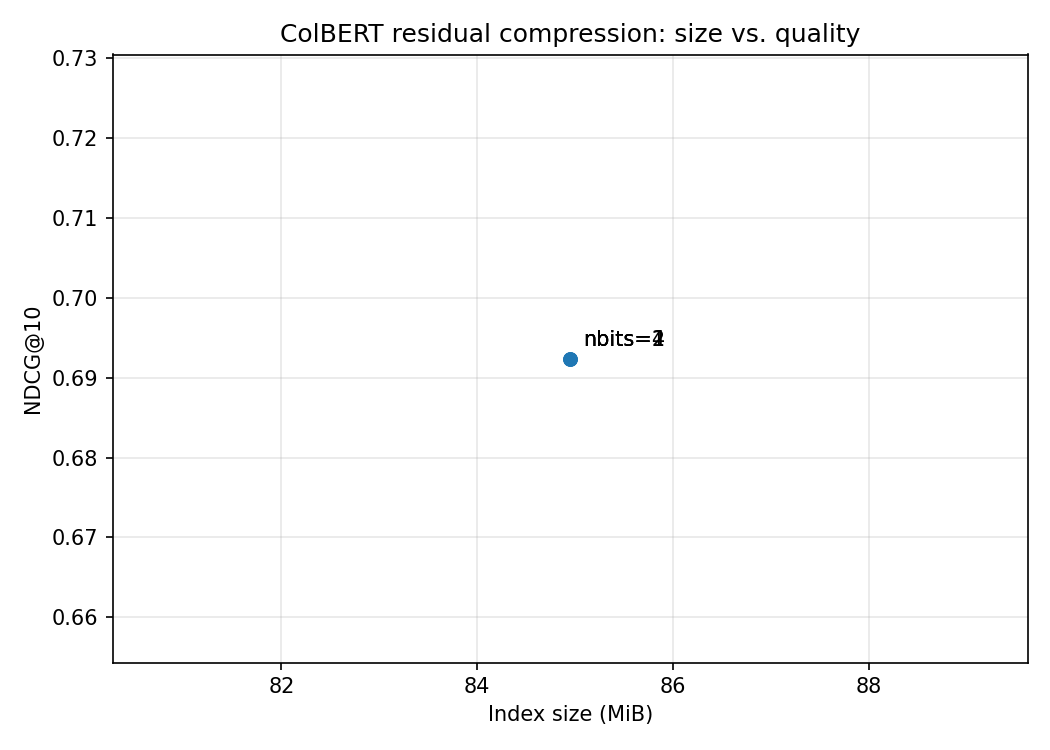
\includegraphics[width=\linewidth]{../results/figures/nbits_size_vs_ndcg.png}
  \caption{SciFact index size vs. NDCG@10 for ColBERTv2 residual compression.}
  \label{fig:nbits}
\end{figure}

\section{Discussion}

The experiment supports a cautious conclusion. ColBERTv2 is better than BM25
on every aggregate metric, which matches the intuition that scientific claims
often require semantic matching rather than exact lexical overlap. At the same
time, the paired significance tests are not strong enough to claim a decisive
win on this 300-query test split.

The residual-compression result is more surprising. After fixing the
RAGatouille wrapper so that \texttt{nbits} is actually written into the
underlying ColBERT config, all three values still produce identical rankings
and index sizes. This suggests that, for a 5,183-document corpus, the tested
compression setting is not the dominant factor controlling effectiveness or
footprint. It may also indicate that other ColBERT/RAGatouille index files
dominate total size at this scale.

RAGatouille was useful, but not completely transparent. It simplified indexing
and search, yet the project still required inspecting the wrapped ColBERT
configuration to ensure the ablation parameter was real. That is the main
engineering lesson from this review: high-level retrieval libraries reduce
boilerplate, but empirical studies still need configuration audits.

\section{Limitations}

This review uses one relatively small benchmark and a pretrained ColBERTv2
checkpoint. We do not fine-tune on SciFact. All ColBERT runs were executed on
macOS without CUDA, so index construction was slow: each full SciFact ColBERT
index took roughly 18--21 minutes to build. A CUDA machine would likely produce
different latency and build-time numbers. Dependency versions also mattered:
RAGatouille 0.0.9 required the older LangChain 0.1 API, so the environment had
to pin \texttt{langchain<0.2}.

\section{Conclusion}

ColBERTv2 is a strong candidate retriever for RAG-style systems because it
keeps token-level semantic matching while remaining indexable. RAGatouille
substantially lowers the implementation burden, but the residual-compression
ablation shows that some internal ColBERT configuration must still be verified
carefully before drawing empirical conclusions.

\begin{thebibliography}{9}

\bibitem{khattab2020colbert}
Omar Khattab and Matei Zaharia. 2020. ColBERT: Efficient and Effective Passage
Search via Contextualized Late Interaction over BERT. In \textit{Proceedings of
SIGIR 2020}. ACM, 727--736.

\bibitem{santhanam2022colbertv2}
Keshav Santhanam, Omar Khattab, Jon Saad-Falcon, Christopher Potts, and Matei
Zaharia. 2022. ColBERTv2: Efficient and Effective Retrieval via Lightweight Late
Interaction. arXiv:2112.01488.

\bibitem{wadden2020scifact}
David Wadden, Shanchuan Lin, Kyle Lo, Lucy Lu Wang, Madeleine van Zuylen, Arman
Cohan, and Hannaneh Hajishirzi. 2020. Fact or Fiction: Verifying Scientific
Claims. In \textit{Proceedings of EMNLP 2020}. ACL, 7534--7550.

\bibitem{thakur2021beir}
Nandan Thakur, Nils Reimers, Andreas Ruckle, Abhishek Srivastava, and Iryna
Gurevych. 2021. BEIR: A Heterogeneous Benchmark for Zero-shot Evaluation of
Information Retrieval Models. In \textit{Proceedings of NeurIPS Datasets and
Benchmarks}.

\bibitem{ragatouille}
Benjamin Clavie. 2024. RAGatouille: Making ColBERT accessible for everyone.
\url{https://github.com/AnswerDotAI/RAGatouille}

\end{thebibliography}

\end{document}
